\documentclass[runningheads,a4paper]{article}
\usepackage[utf8]{inputenc}
\setcounter{tocdepth}{3}
\usepackage[english]{babel} 
\usepackage{graphicx}
\usepackage{grffile}
\usepackage{float}
\usepackage{multicol}
\usepackage{url}
\usepackage{titling}
\usepackage[hidelinks]{hyperref}
\setcounter{secnumdepth}{5}
%Margins
\usepackage[
margin=2cm,
includefoot
]{geometry}
\graphicspath{{img/}}
%Headers and Footers
\usepackage{fancyhdr}
\pagestyle{fancy}
\fancyhead{}
\fancyfoot{}
\fancyfoot[R]{\thepage}
\renewcommand{\headrulewidth}{0pt}
\renewcommand{\footrulewidth}{0pt}
\setlength\parindent{24pt}
\begin{document}
%Title Page
\begin{titlepage}
\begin{center}

\includegraphics[width=10cm]{UP.jpg}  \\
[1cm]
\line(1,0){300} \\
[0.3cm]
\textsc{\Large
NavUP \\
Architectural Requirements Specifications and Design \\
\hfill \break 01 March 2017
%University of Pretoria
}\\
[0.1cm]
\line(1,0){300} \\
[0.7cm]
\textsc{\Large
Team MatLab
} \\
\end{center}
\begin{center}
\begin{multicols}{2}
\textsc{\large\\
Frederick Ehlers\\ 
u11061112\\ 
}
\textsc{\large\\
Vignesh Iyer\\
u15031625\\ 
}
\textsc{\large\\
Stephanie Groutsch\\
u14293324\\ 
}
\textsc{\large\\
Neo Thokoa\\
u14163285\\
}
\columnbreak
\textsc{\large\\
Nokuthula Manana\\
u12064115\\
}
\textsc{\large\\
Jacobus Marais\\
u15188397\\
}
\textsc{\large\\
Heinrich Burgers\\
u15059538\\
}
\end{multicols}
\textsc{	\\ \href{https://github.com/FredJEhlers/Matlab}{GitHub}
\url{https://github.com/FredJEhlers/Matlab}}
\end{center}
\end{titlepage}

%\maketitle



\begingroup



\tableofcontents

\addcontentsline{toc}{section}{Table Of Contents}

\endgroup

\newpage




\section{External Interface Requirements}
\subsection {Navigation}
The navigation system communicates to three main entities. The network, the user and the user’s device. There needs to be an interface 
between each one of these entities to allow communication. 

User interface: 
The user interacts with the navigation system via the GUI. This GUI needs to be flexible enough to function on devices of various sizes 
and operating systems. The interface must allow the user to have some method of control over the navigation system like choosing 
destinations, waypoints, routes and change in these routes. 

The navigation system should also communicates to the user by showing information on the screen and through audio. This information
includes messages on the screen, the map, locations on the map and the possible routes on the map.

Other aspects of the user interface like font, icons and the more visual aspects will be decided upon when the GUI is created.

Device Interface:
In order to allow communication between the device and the navigation system an interface needs to be created. The navigation system 
needs access and information from the device in order to function. This includes access to its hardware like the screen, 
device memory, connection to Wi-Fi or the internet, the location system and to information like the device identity. 

The navigation system will be installed on the device along with the application. Being on the device itself will give it the needed
access, if permission was granted. 

Network Interface:
The navigation system functions best with communication between it and the network. This connection is established through the device’s 
connection. The connection can be to a WI-FI network or the mobile data network. 

The interface needs to facilitate exchange of information like location, identity, traffic, route information and aspects that might 
influence how navigation will take place. These aspects can be events, personal preference or personal 
information like disabilities. 



\section{Performance Requirements}



\section{Design Constraints}



\section{Software System Attributes}



\section{UML Diagrams for the Chosen Subsystems}

Design Patterns have been integrated and a discussion of their use are made below the respective diagrams.


\begin{figure}[H]
   	\centering
   	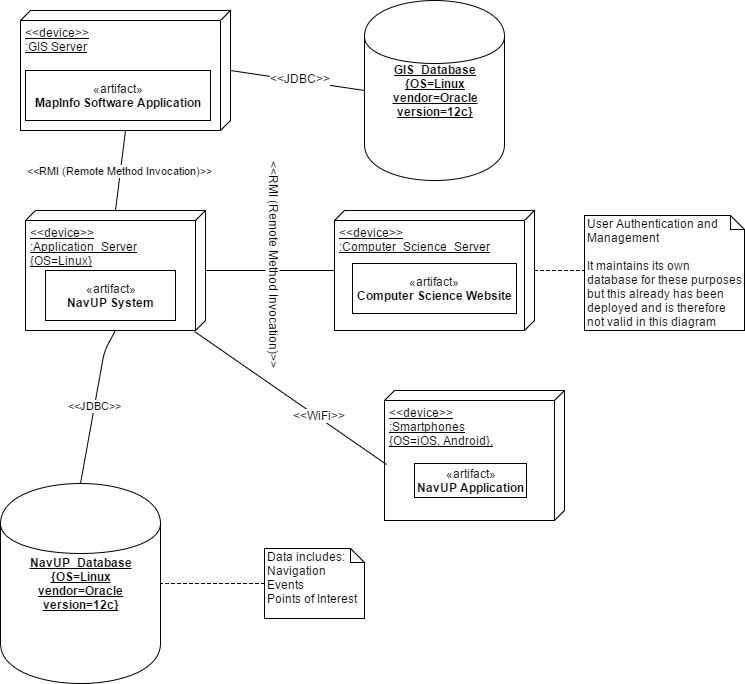
\includegraphics[width=0.7\textwidth]{DeploymentDiagram.jpg}
   	\caption{Deployment Diagram for NavUP}
\end{figure}


\subsection {User}

\begin{figure}[H]
   	\centering
   	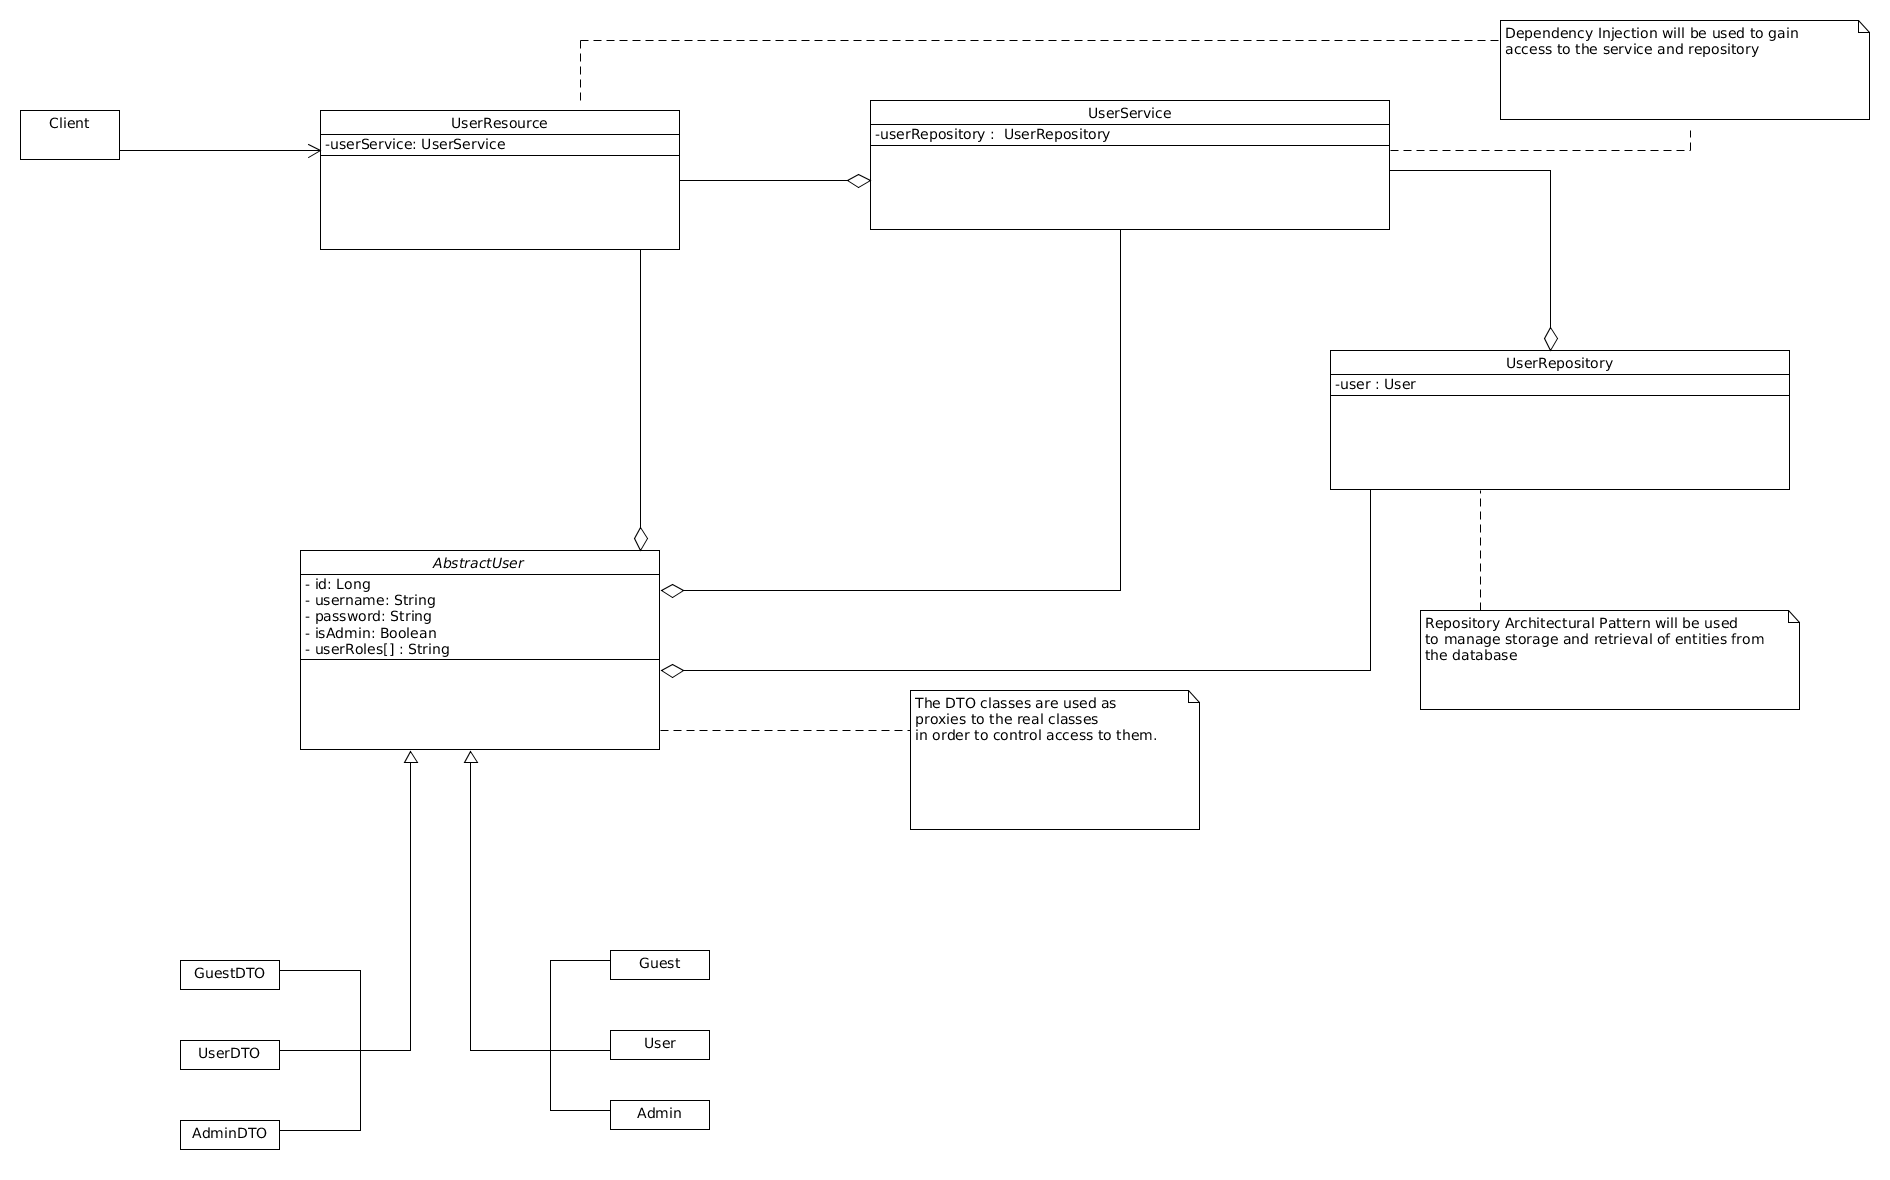
\includegraphics[width=0.7\textwidth]{User_Class_Diagrams.png}
   	\caption{Class Diagram for the User Module}
\end{figure}
\subsubsection {Explanation of Design Patterns in User Module}
\begin{itemize}
\item \underline{Proxy Pattern} The Proxy pattern has been used in the users module in order to control access to the user profiles within the backend application. By doing this we add a wrapper and delegation to protect the real component from complexity. 

\item The Data Transfer Objects (DTO's)  can have extra / less fields depending on what the client is or is not allowed to see in the user object. Typically the user object will have more fields than the DTO ( such as roles, hashes of passwords etc). 

\item \underline{Repository Pattern} The Repository Architectural Pattern will be used to manage database access. This pattern enables direct mapping of database objects / row entries to classes. It also delegates the responsibilty of managing the database to a single object. Listed below are a few advantages of using the Repository pattern:
	\begin{itemize}
		\item Enables one to maximize the amount of code that can be tested and isolate the data layer to support unit testing. 
		\item Enable one to access the data source from many locations by using dependency injection as well as apply centrally managed, consistent access rules and logic.
		\item Improve maintainability and readability of code by separating business logic from data access logic.  
	\end{itemize}

 
\end{itemize}

\subsection {Navigation}

\begin{figure}[H]
   	\centering
   	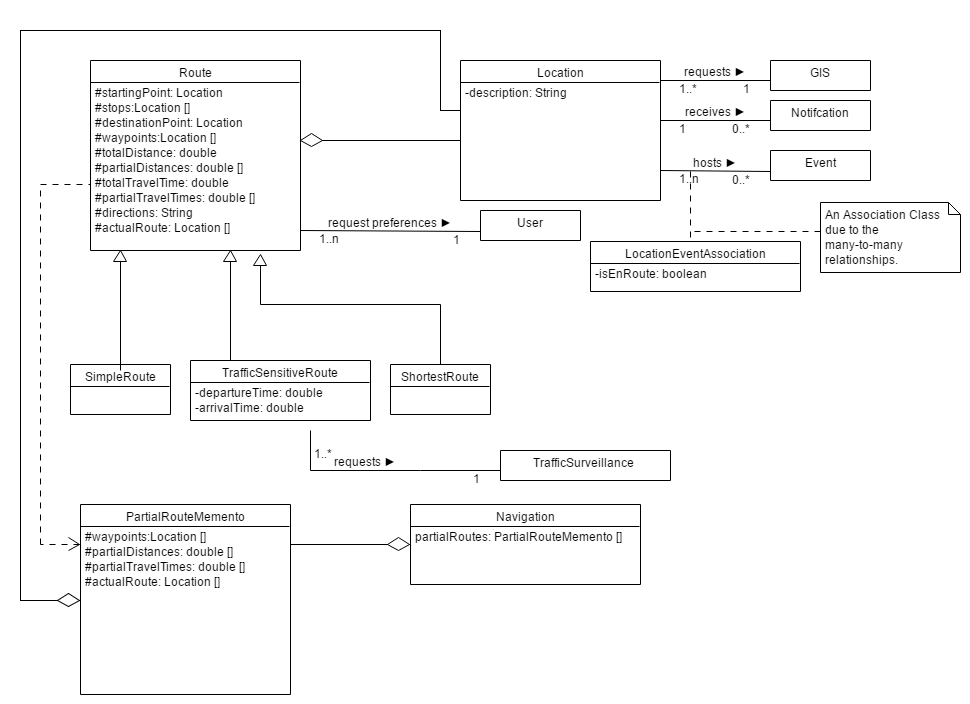
\includegraphics[width=0.7\textwidth]{Navigation-Module-Class-Diagram.png}
   	\caption{Class Diagram for the Navigations Module}
\end{figure}

\subsubsection {Explanation of Design Patterns in Navigation Module}
\begin{itemize}

\item \underline{Memento Pattern} - The Memento Pattern has been used in the navigation module in order to capture the internal state of a "route" object while the route is being calculated.
\item The internal state of the route that we would like to capture is the respective arrays for waypoints, partial distances, partial times and actual distances in the route. 
\item While routing, connection can be lost or the user may diverge from the specified paths during which the system will have to save the internal state so that it can return to this state at a later stage.
\item The role-back function in this case would be the re-route function.
\item The originator in the module is the Route class.
\item The caretaker is the Navigation class.
\item The memento is the PartialRouteMemento class.

\item \underline{Strategy Pattern} - The Strategy Pattern has been used in the navigation module in order to define a family of routing algorithms and make them interchangeable.
\item The users of the system will specify by clicking on different icons, the type of routing they want.
\item The abstraction class would be the Route class which is the interface to the user and is very generic with fundamental functionality.
\item The implementation classes would be the SimpleRoute, ShortestRoute and TrafficSenstiveRoute classes that will override the functionality of the superclass with algorithms for their respective needs.

\end{itemize}

\begin{figure}[H]
   	\centering
   	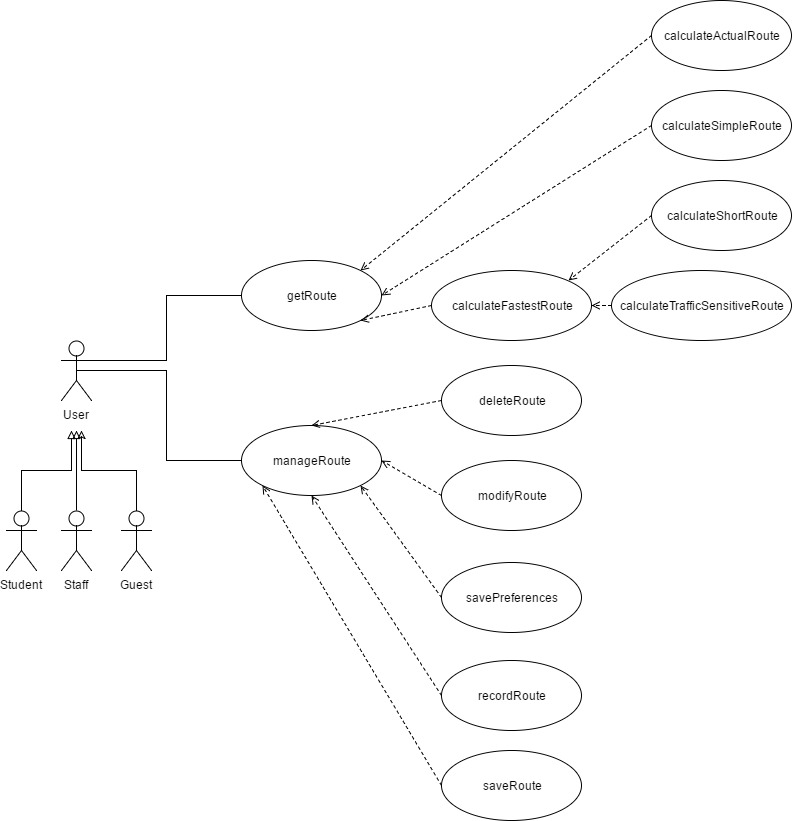
\includegraphics[width=0.7\textwidth]{Navigation-Module-Use-Case.jpg}
   	\caption{Use Case Diagram for the Navigations Module}
\end{figure}


\subsection {Notifications}



\subsubsection{External Interface Requirements}



\paragraph{Software Interface}
\mbox{}\\
The mobile application will connect to the database in order to obtain the users’ information. One such example includes obtaining information regarding the individuals selected notification medium. The mobile application will also connect to the server in order to update information regarding the users email address and mobile number.

\mbox{}\\
The server will be connected to the notification plugins, which include email and SMS plugins, as well as the application itself in times when notifications are displayed as a pop-up on the users’ mobile device.



\paragraph{Hardware Interface}

\mbox{}\\
The user will interact with the mobile device screen in order to set their notification medium preference that is sent and stored on the server. 

\mbox{}\\
When there is a notification, the server will then send data packets to the mobile application by making use of sockets. This will cause the mobile device to display the message as well as vibrate or make a sound. 

\mbox{}\\
The user will once again interact with the screen on their mobile device in order to view the notification.

\paragraph{User Interface}
\mbox{}\\
The user will initially interact with the notifications module through the application’s GUI where they will request to be notified about a certain event as well as provide their chosen notification medium. 

\mbox{}\\
If the chosen notifications medium is email, the user will receive a generic email with the given notification. The email will provide a description of the notification in its title. If required, the email will provide a link to the relevant website for more information concerning the notification. If the user selected to receive notifications via SMS, a message describing the notification will be sent to each user. Once again, a link will be provided in the SMS for more information concerning the notification as required. If the user decided to receive notifications through the application, a pop-up will appear on the applications’ GUI when there is a notification. 

\subsubsection{Performance Requirements}

The system should be able to send out a large number of notifications without any delay (within 5 seconds).\\

Multiple administrators should be able to add new notifications without failure.



\subsubsection{Design Constraints}



\subsubsection{Software System Attributes}
\begin{enumerate}

\item[•] Flexibility: The system should allow for the addition of new notification means.
\item[•]Maintainability: The users’ contact information should be updated on a regular basis.
\item[•]Security: The users’ contact information should be kept secure in order to ensure that third parties do not have access to it.
\item[•]Auditability: The system should keep track of the sent and requested notifications.
\item[•]Integrability: The system should allow for future expansions.

\end{enumerate}



\subsubsection{UML Diagrams}
\paragraph{Class Diagram}
\begin{center}
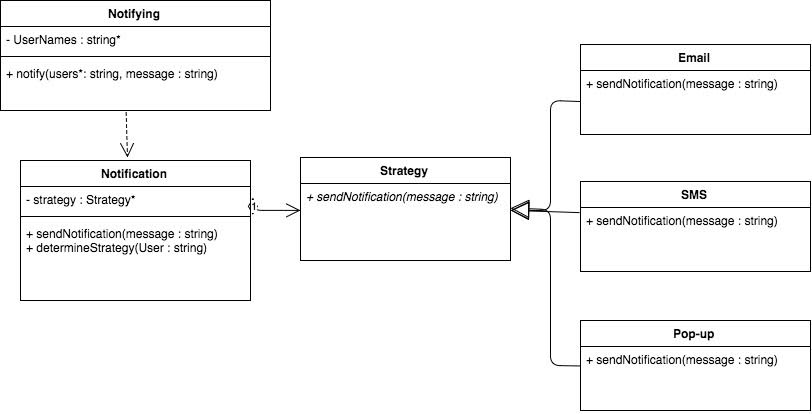
\includegraphics[width=10cm]{ClassDiagram.png}\\
\end{center}
\paragraph{Activity Diagram}
\begin{center}
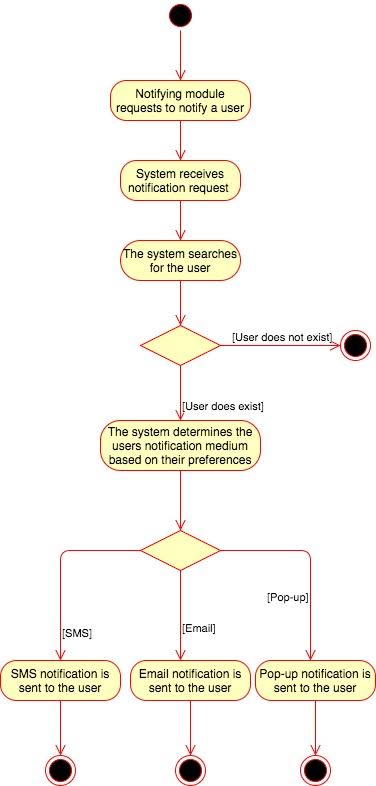
\includegraphics[height=10cm,width=5cm]{ActivityDiagram.png} 
\end{center}



\subsubsection{Technology Choices}



\subsection {Point of Interest}



\section{Technology Choices}



\section{References}

Kung, D.C. (2013) Object-oriented software engineering: An agile unified methodology. New York: McGraw Hill Higher Education.



\end{document}